
\section{Method}
\label{sec:method}

% Include exp_setup.jpg figure
\begin{figure}
    \centering
    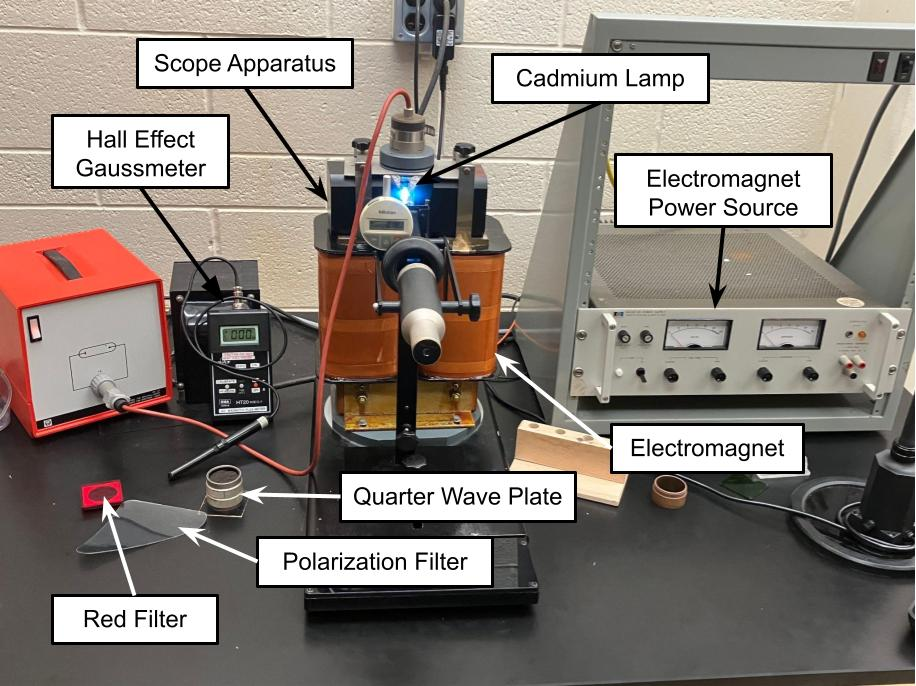
\includegraphics[width=0.8\textwidth]{method/labeled_diagram.jpg}
    \caption{Picture of Experimental Setup.}
    \label{fig:exp_setup}
\end{figure}

\begin{figure}
    \centering
    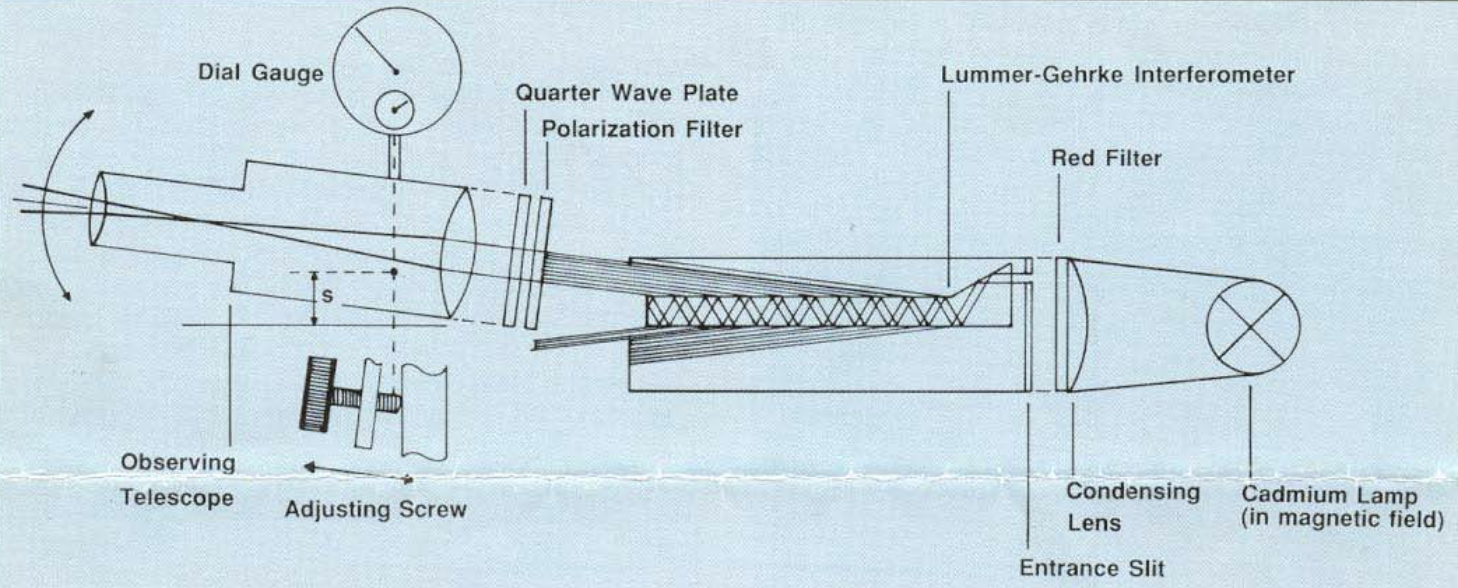
\includegraphics[width=0.8\textwidth]{method/setup_diagram.png}
    \caption{Diagram of Experimental Setup. \cite{ZeemanEffectLab}}
    \label{fig:diagram_setup}
\end{figure}

For the experiment we are provided with a mercury lamp, a power supply, a dial gauge, a Hall probe, and an electromagnet. The mercury lamp is used as a source of light, and the dial gauge is used to measure the position of the spectral lines. The Hall probe is used to measure the magnetic field strength at the center of the electromagnet, and the power supply is used to supply the current to the electromagnet. The electromagnet is used to create a magnetic field perpendicular to the light source. The experimental setup is shown in Figure \ref{fig:exp_setup}.
Figure \ref{fig:diagram_setup} shows a diagram of the experimental setup.

The experiment is divided into three sections:

\subsection{Part 1: Magnetic field strength and current}
In the first part of the experiment, we measure the magnetic field strength as a function of the current supplied to the electromagnet. We do this by measuring the magnetic field strength at the center of the electromagnet using a Hall probe and the current as the current from the power source. We measure the magnetic field strength at about 10 different current values, and then fit the data to a linear model and an exponential model to determine the best relationship between the current and the magnetic field strength.

\subsection{Part 2: Observing the Zeeman split perpendicularly to the magnetic field with different field values}

Next, we measure how the Zeeman split changes with different magnetic field values.
We do this by measuring the width of the spectral lines of the mercury lamp with and without a magnetic field.
We then calculate the Zeeman shift for each trial.

First, without the field turned on, we measure the position given by the dial gauge for a number of lines.
Then, we turn on the magnetic field and measure the upper and lower bounds of each line. Because
the lines do not appear to perfectly separate, and only a widening of the lines can be observed,
we measure the top most and bottom most points of the line, and calculate the width of the line as the difference between the two.


with respect to the field strength

The Zeeman shift values from the previous part are plotted against a linear fit. We graph the best fit relationship and
evaluate the goodness of fit criteria to determine how well the linear model matches the experimental results.


\subsection{Part 3: measuring the $\frac{e}{m}$ relationship.}

Finally, from the slope of the best fit line obtained in the previous part, we determine the
experimental value for the $\frac{e}{m}$ ratio of the electron by using the average line separation from all our trials using equation \ref{eq:em_relationship}. We compare this value to the accepted value.

\subsection{Part 4: Polarization of the emitted light}

We explore the polarization of the emitted light in two different orientations.

First, we start from the setup where the electric field is perpendicular to the lens (as in Figure \ref{fig:diagram_setup}).
We insert the circular polarization filter in the socket on the lens, and rotate it to observe different kinds of polarization.

We then rotate the apparatus so that the electric field is parallel to the lens.
Likewise, we attempt to observe the polarization of the Zeeman split lines through a small opening in one of the electromagnets.